\documentclass[paper=a4, fontsize=11pt]{scrartcl}
\usepackage[pdftex]{graphicx}
\usepackage[utf8x]{inputenc}
\usepackage[portuges,brazilian]{babel}
\usepackage{amsmath,amsfonts,amsthm,mathtools} % Math packages
\usepackage{hyperref}
\usepackage{indentfirst}
\usepackage{float}
\usepackage{caption}
\usepackage{subcaption}
\usepackage{todonotes}
%\usepackage{biblatex}
%\usepackage{natbib}
\selectlanguage{brazilian}
\usepackage{fancyhdr}
\pagestyle{fancyplain}
\fancyhead{}											% No page header
\fancyfoot[L]{}											% Empty 
\fancyfoot[C]{}											% Empty
\fancyfoot[R]{\thepage}									% Pagenumbering
\renewcommand{\headrulewidth}{0pt}			% Remove header underlines
\renewcommand{\footrulewidth}{0pt}				% Remove footer underlines
\setlength{\headheight}{13.6pt}

%%% Equation and float numbering
\numberwithin{equation}{section}		% Equationnumbering: section.eq#
\numberwithin{figure}{section}			% Figurenumbering: section.fig#
\numberwithin{table}{section}				% Tablenumbering: section.tab#


%%% Maketitle metadata
\newcommand{\horrule}[1]{\rule{\linewidth}{#1}} 	% Horizontal rule

\title{
		%\vspace{-1in} 	
		\usefont{OT1}{bch}{b}{n}
		\normalfont \normalsize \textsc{Pontíficia Universidade Católica do Rio de Janeiro \\ Departamento de Engenharia Elétrica} \\ 
		\horrule{0.5pt} \\[0.4cm]
		\huge Regressão Quantílica \\
		\horrule{2pt} \\[0.5cm]
}
\author{
		\normalfont 								\normalsize
        Henrique Helfer Hoeltgebaum\footnote{Aluno de doutorado do Departamento de Engenharia Elétrica da PUC-RIO.}~,
        Marcelo Castiel Ruas\footnote{Aluno de doutorado do Departamento de Engenharia Elétrica da PUC-RIO.}~,
         Alexandre Street\footnote{Professor do Departamento de Engenharia Elétrica da PUC-RIO.}~,\\ \normalfont 								\normalsize Cristiano Fernandes\footnote{Professor do Departamento de Engenharia Elétrica da PUC-RIO.}\ 
        \\[-1pt]		\normalsize
        \today}

\date{}
\setlength\parindent{24pt}
\begin{document}

\maketitle
\section{Introdução}\label{intro}
A previsão da maioria dos modelos de regressão é apenas uma estimativa da média condicional da variável resposta, para um dado conjunto de preditores. Porém, a média condicional representa apenas a medida de tendência central da distribuição da variável resposta. Um quadro mais completo a respeito da relação entre a distribuição condicional da variável dependente com a das independentes pode ser obtido pelos seus quantis. Recentes avanços em computação tornaram viáveis o desenvolvimento de modelos de regressão para prever um dado quantil da distribuição condicional, tanto parametricamente quanto não parametricamente. Tal metodologia é chamada de Regressão Quantílica, mas a metodologia (da estimação do quantil condicional) se aplica para qualquer modelo estatístico.

%%%%%%%%%%%%%%%%%%%%%%%%%%%%%%%%%%%%%%%%%%%%%%%%%%%%%%%%%%%%%%%%%%%%%%%%%%%%%%%%%%%%%%%%%%%%%%%%%%%%%%%%%%%%%%%%%%%%%%%%%%%%%%%%%%%%%%%%%%%%%%%%%%%%%%%%%%%%%%%%%%%%%%%%%%%

\section{Regressão Quantílica}\label{regQuantilica}
Em um modelo de regressão simples via mínimos quadrados ordinários (OLS), modelamos a média condicional da variável resposta (ou dependente) como função de uma ou mais variáveis independentes. Mas, como a média não é uma descrição completa da distribuição, modelar a média não resulta em uma descrição completa da relação entre a variável dependente e as respectivas variáveis independentes, logo essa análise pode não ser adequada.

Para enfatizar a necessidade de tal análise, cita-se um simples exemplo, supondo que nossa variável dependente seja bimodal ou multimodal, isto é, possui múltiplos picos conforme ilustrado pela Figura~\ref{fig:densidades}.

\begin{figure}[H]
%\centering
\begin{subfigure}{.5\textwidth}
  \centering
  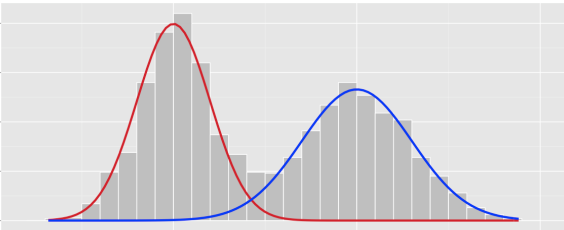
\includegraphics[width=75mm]{Figuras/bimodal.png}
  \caption{Distribuição Bimodal}
  \label{fig:bimodal}
\end{subfigure}%
\begin{subfigure}{.5\textwidth}
  \centering
  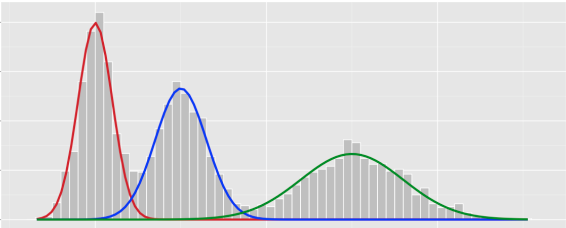
\includegraphics[width=75mm]{Figuras/multimodal.png}
  \caption{Distribuição Multimodal}
  \label{fig:multimodal}
\end{subfigure}
\caption{Gráficos das densidades de distribuições bimodais e multimodais}
\label{fig:densidades}
\end{figure}

Se soubermos o que causa a bimodalidade, podemos separar aquela variável e prosseguir com uma análise estratificada, porém caso não conhecermos, o arcabouço dos modelos de regressão quantílica se demonstram uma alternativa eficaz para tal análise. Uma vez que a regressão por mínimos quadrados, nesse caso pode causar resultados não confiáveis dado que esta se apoia na média como uma medida central para uma distribuição bimodal.

Além do exemplo supracitado, a regressão quantílica traz um  resumo de informações muito mais completo, com relações interessantes que podem ser obtidas através dos quantis da distribuição condicional da variável resposta. Quando existe o interesse em saber, por exemplo, relações entre as pessoas com maior e menor renda, conforme será apresentado na Seção~\ref{estimacao}, cada parâmetro dos regressores são estimados como função do quantil a ser estudado, nesse caso estudaríamos os quantis \{0.05,0.95\} da distribuição da variável dependente \emph{renda} com suas covariáveis, tendo para cada quantil $\tau$ um respectivo $\hat{\beta_{i}}(\tau)$.

Ou seja, ao invés do modelo de regressão linear estimado via mínimos quadrados ordinários,
\vspace{-10pt}
\begin{align} 
	\begin{split}
	y_{i} = \beta_{0} + \beta_{1}x_{i1} + \beta_{2}x_{i2} + ... + \beta_{in}x_{n} + \varepsilon_{i} \label{eq:1}
	\end{split}					
\end{align}

{\parindent0pt teremos o seguinte modelo de regressão quantílica, que fornece os quantis condicionais de $y$ por meio da seguinte equação,}

\vspace{-10pt}
\begin{align} 
	\begin{split}
	Q_{y}(\tau|x_{1}, x_{2}, ..., x_{n}) = \beta_{0}(\tau) + \beta_{1}(\tau)x_{1} + \beta_{2}(\tau)x_{2} + ... + \beta_{n}(\tau)x_{n} + \emph{F}^{-1}_\varepsilon(\tau) \label{eq:2}
	\end{split}					
\end{align}

{\parindent0pt onde $\emph{F}_\varepsilon$ indica a função distribuição dos erros.}

%%%%%%%%%%%%%%%%%%%%%%%%%%%%%%%%%%%%%%%%%%%%%%%%%%%%%%%%%%%%%%%%%%%%%%%%%%%%%%%%%%%%%%%%%%%%%%%%%%%%%%%%%%%%%%%%%%%%%%%%%%%%%%%%%%%%%%%%%%%%%%%%%%%%%%%%%%%%%%%%%%%%%%%%%%%

\subsection{Estimação dos parâmetros}\label{estimacao}
Conforme apresentado na Seção 1.3 de~\cite{koenker2005quantile}, os pontos discutidos de que os quantis podem ser expressos como solução de um simples problema de otimização leva, naturalmente, a métodos mais gerais de estimação de modelos de quantil condicional. Mínimos quadrados oferecem o referido arcabouço para esse desenvolvimento. Sabendo que a média amostral resolve o problema
\vspace{-10pt}
\begin{align} 
	\begin{split}
	\underset{\mu \; \in \; \mathbb{R} }{\text{min}} \sum_{i=1}^{n} (y_{i}-\mu)^{2} \label{eq:3}
	\end{split}					
\end{align}
{\parindent0pt sugerindo que, se desejamos expressar a média condicional de $y$ dado $x$ como $\mu(x)=x^{T}\beta$, então $\beta$ pode ser estimado resolvendo}
\vspace{-10pt}
\begin{align} 
	\begin{split}
	\underset{\beta \; \in \; \mathbb{R}^p }{\text{min}} \sum_{i=1}^{n} (y_{i}-x_{i}^{T}\beta)^{2}. \label{eq:4}
	\end{split}					
\end{align}

Similarmente, uma vez que o $\tau$-ésimo quantil amostral, $\hat{\alpha}(\tau)$ resolve
\vspace{-10pt}
\begin{align} 
	\begin{split}
	\underset{\alpha \; \in \; \mathbb{R} }{\text{min}} \sum_{i=1}^{n} \rho_{\tau}(y_{i}-\alpha). \label{eq:5}
	\end{split}					
\end{align}

{\parindent0pt somos levados a especificar o $\tau$-ésimo quantil condicional como $ Q_{y}(\tau|x)=x^{T}\beta(\tau) $, e para a estimação de $ \hat{\beta}(\tau) $ basta resolver}
\vspace{-10pt}
\begin{align} 
	\begin{split}
	\underset{(\beta,u,v) \; \in \; \mathbb{R}^{p} }{\text{min}} \sum_{i=1}^{n} \rho_{\tau}(y_{i}-x_{i}^{T}\beta). \label{eq:6}
	\end{split}					
\end{align}

Esta é a idéia principal apresentada com maiores detalhes em \cite{koenker1978regression}.

O problema de regressão quantílica apresentado pela Equação~\eqref{eq:6} pode ser reformulada como um problema de programação linear,

\vspace{-10pt}
\begin{align} 
	\begin{split}
	\underset{\beta \; \in \; \mathbb{R}^{p} \times \mathbb{R}^{2n}_{+} }{\text{min}} \{\tau \mathbf{1}_{n}^{T}u + (1-\tau)\mathbf{1}_{n}^{T}v | X\beta + u - v = y \} ,\label{eq:7}
	\end{split}					
\end{align}

{\parindent0pt onde $ X $ representa a matriz usual dos regressores n por p. Divide-se o vetor de resíduos $ y-X\beta $ em partes negativas e positivas ($u$ e $v$), e então estamos minimizando uma função linear em um poliedro restrito por um conjunto de restrições, e muitas das propriedades importantes das soluções, $\hat{\beta(\tau)}$, os quais são denominamos "quantis regressores", são derivadas imediatamente a partir de propriedades de soluções bem conhecidas de problemas lineares. }


%%%%%%%%%%%%%%%%%%%%%%%%%%%%%%%%%%%%%%%%%%%%%%%%%%%%%%%%%%%%%%%%%%%%%%%%%%%%%%%%%%%%%%%%%%%%%%%%%%%%%%%%%%%%%%%%%%%%%%%%%%%%%%%%%%%%%%%%%%%%%%%%%%%%%%%%%%%%%%%%%%%%%%%%%%%
\subsection{Seleção do modelo}
Conforme apresentado na Seção 4.9.1 de \cite{koenker2005quantile}, existe uma vasta literatura a respeito de seleção de modelos. Serão abordados apenas alguns desenvolvimentos recentes a cerca do tema. 

Em \cite{machado1993robust} é apresentada uma variação do critério de penalização de Schwarz para M-estimadores de regressão, incluindo o caso da regressão quantílica. É enfatiza a necessidade de procedimentos invariantes a locação e escala: para regressões da mediana ($\tau$=1/2) o seguinte cálculo rende o critério,
\vspace{-10pt}
\begin{align} 
	\begin{split}
	SIC(j) = log(\hat{\sigma}_{j})+\frac{1}{2}p_{j}\;log\;n,\label{eq:SIC}
	\end{split}					
\end{align}

{\parindent0pt onde $\hat{\sigma}_{j}=\sum_{i=1}^{n} \rho_{1/2}(y_{i}-x^{T}_{i}\hat{\beta}_{n}(1/2))$ e $p_{j}$ indica a dimensão do $j$-ésimo modelo. Esse procedimento rende uma seleção de modelo consistente sob a circustância de que um dos modelos $p_{j}$-dimensional esteja de fato bem especificado.}

Alternativamente ao critério supracitado, podemos considerar o critério de Akaike, calculado conforme
\vspace{-10pt}
\begin{align} 
	\begin{split}
	AIC(j) = log(\hat{\sigma}_{j})+p_{j}.\label{eq:AIC}
	\end{split}					
\end{align}
Com prababilidade positiva, a seleção baseada na minimização do AIC($j$) superestima a dimensão do modelo, mas pode vir a exercer uma performance superior para a previsão. 

%%%%%%%%%%%%%%%%%%%%%%%%%%%%%%%%%%%%%%%%%%%%%%%%%%%%%%%%%%%%%%%%%%%%%%%%%%%%%%%%%%%%%%%%%%%%%%%%%%%%%%%%%%%%%%%%%%%%%%%%%%%%%%%%%%%%%%%%%%%%%%%%%%%%%%%%%%%%%%%%%%%%%%%%%%%

\subsection{Diagnósticos}
Em \cite{koenker1999goodness} é apresentada uma versão do familiar $ R^{2} $ do modelo de regressão por mínimos quadrados para o modelo de regressão quantílica, o $ R^{1}(\tau) $. Atenta-se ao fato de que esse novo parâmetro é uma medida de diagnóstico para um quantil em particular, ao contrário do seu análogo $ R^{2} $ que fornece uma medida global de ajuste sob toda a distribuição condicional. É fácil de imaginar circunstâncias na qual as covariáveis podem exercer um efeito em uma cauda da distribuição condicional da variável resposta porém podem vir a não surtir efeito na outra cauda. Em \cite{chamberlain1994quantile} é apresentado um exemplo disso no arcabouço de regressão quantílica. 

Alternativamente à metodologia supracitada, em \cite{van2007worm} (Seção 5), é apresentada uma ferramenta de diagnóstico visual para verificar o ajuste do modelo aos dados. Essa metodologia é denominada de "gráfico da minhoca", nela é possível apontar os quantis nos quais o ajuste pode ser melhorado e comparar o ajuste de diferentes modelos com o modelo selecionado. 

%%%%%%%%%%%%%%%%%%%%%%%%%%%%%%%%%%%%%%%%%%%%%%%%%%%%%%%%%%%%%%%%%%%%%%%%%%%%%%%%%%%%%%%%%%%%%%%%%%%%%%%%%%%%%%%%%%%%%%%%%%%%%%%%%%%%%%%%%%%%%%%%%%%%%%%%%%%%%%%%%%%%%%%%%%%
%---------------------------------------------------------------------------------------------------------------------------------------------------------------------------------------------%
%------------------------------------------------------PAREI AQUI! Daqui para baixo----------------------------------------------------------------------------------------------------------------%
%---------------------------------------------------------------------------------------------------------------------------------------------------------------------------------------------%

\subsection{Previsão fora da amostra}

\todo[inline]{Escrever sobre previsão pontual e densidade preditiva}
% googleia out of sample forecast quantile regression
% paper erik bunn --> descrição muito boa de regressão quantílica!
%http://astrostatistics.psu.edu/datasets/R/html/quantreg/html/predict.rq.html
%http://faculty.washington.edu/marzban/quantile.pdf


%---------------------------------------------------------------------------------------------------------------------------------------------------------------------------------------------%
%------------------------------------------------------PAREI AQUI! Daqui para baixo----------------------------------------------------------------------------------------------------------------%
%---------------------------------------------------------------------------------------------------------------------------------------------------------------------------------------------%

\section{Regressão Quantílica para séries temporais}\label{regQuantilicaST}
Quando relaxada a condição de independência das observações, podemos continuar com a aplicação da metodologia de regressão quantílica. Bloomfield e Steiger (1983) mostraram a normalidade assintótica de um estimador autoregressivo da mediana para um modelo no qual as observações $\{(x_{i},y_{i}):i=1,...,n\}$ eram assumidas serem estacionárias e de diferença martingal ergódiga.

\subsection{Autoregressão}
Já existe uma ampla literatura a respeito da estimação e inferência para modelos de séries temporais lineares se utilizando de métodos de regressão quantílica. Bloomfiel e Steiger (1983) consideraram o modelo autoregressivo
\vspace{-10pt}
\begin{align} 
	\begin{split}
	y_{t}=\alpha_{0}+\alpha_{1}y_{t-1}+...+\alpha_{p} y_{t-p}+u_{t} \label{eq:modelo_AR}
	\end{split}					
\end{align}

{\parindent0pt com a condição usual de estacionariedade de que as raízes do polinômio característico $1-\alpha_{1}z-...-\alpha_{p}z^{p}=0$ permaneçam fora do círculo unitário e com erros $u_{t}$ iid com uma distribuição nonlattice $F$ satisfazendo as seguintes condições: (i) $E(log_{+}|{u_{t}|})$}, (ii) mediana $\{u_{t}\}$=0, e (iii) $E|u_{t}| < \infty$. Isso prova que o estimador da regressão da mediana
\vspace{-10pt}
\begin{align} 
	\begin{split}
	\hat{\alpha_{n}}=argmin_{\alpha \in \mathbb{R}} \sum_{t=1}^{n}|y_{t}-\alpha_{0}-\alpha_{1}y_{t-1}-...-\alpha_{p} y_{t-p}|  \label{eq:modelo_AR}
	\end{split}					
\end{align}

{\parindent0pt É fortemente consistente. Quando $F$ tem densidade $f(0)>0$, e $Eu_{t}^2=\sigma^2<\infty$, as técnicas descritas anteriormente (veja Poolard, 1991, Exemplo 2) podem ser usadas para estabelecer normalidade assintótica de $\hat{\alpha_{n}}(\tau)$.}

É valido considerar um simples modelo AR(1) a fim de ilustração,
\begin{align} 
	\begin{split}
	y_{t}=\alpha_{1}y_{t-1}+u_{t} \label{eq:modelo_AR_1},
	\end{split}					
\end{align}
{\parindent0pt demonstraremos algumas características especiais da especificação AR. Considerando $n^{-1}\sum y_{t-1}^2 \rightarrow \frac{\sigma^2}{(1-\alpha^2)}$ e utilizando a quantidade que podemos denominar de $D_{0}$ para enfatizar a analogia com o caso de regressão, é fácil mostrar que}
\begin{align} 
	\begin{split}
	\sqrt n (\hat{\alpha_{n}}-\alpha) \leadsto N(0,\omega^{2}D_{0}^{-1})
	\end{split}					
\end{align}
 {\parindent0pt onde $\omega = (2f(0))^{-1}$. Em contraste, o estimador de mínimos quadrados de $\alpha$,}
\begin{align} 
	\begin{split}
	\tilde{\alpha_{n}}=\frac{\sum_{t=2}^{n}y_{t}y_{t-1}}{\sum_{t=2}^{n}y_{t-1}^2}
	\end{split}					
\end{align}     
{\parindent0pt satisfaz, sob a condição de que,}
\begin{align} 
	\begin{split}
	\sqrt n (\tilde{\alpha_{n}}-\alpha) \leadsto N(0,\sigma^{2}D_{0}^{-1})
	\end{split}					
\end{align}   
 
\subsection{Modelos ARMA}
Segundo a Seção 2.6.2 de \cite{koenker2005quantile} os modelos autoregressivos se ajustam bem ao arcabouço original da regressão quantílica: a computação é direta e muitas das propriedades da teoria assintótica de regressão se mantém.

No caso dos modelos ARMA, a situação é complicada pela não convexidade da função objetivo, uma dificuldade que é superada pela aproximação criteriosa da função objetivo na vizinhança do verdadeiro valor do parâmetro. Isso assegura uma sequência de minimizadores $locais$ que convergem como especificados mas também implica em alguma preocupação a respeito dos métodos computacionais que irão levar ao minimizador apropriado. 

Até hoje, grande parte da literatura de aplicações de regressão quantílica em séries temporais foca em modelos com inovações iid. Parece haver um escopo considerável para explorar modelos que partem dessa condição restritiva. Os primeiros passos nessa direção são descritos na Seção 8.3 de \cite{koenker2005quantile}, através da exemplificação dos modelos QAR que será discutido na próxima Seção \ref{QAR}.

\subsection{Modelos QAR}\label{QAR}
Existe uma ampla literatura a respeito dos modelos QAR. Nesse modelo o $\tau$-ésimo quantil condicional da variável resposta $y_{t}$ é expressado como uma função linear de valores defasados da resposta. Mas uma característica notável a respeito dessa literatura é que ela tenha se focado, quase que exclusivamente em inovações iid, na qual as variáveis condicionantes possuem um papel de deslocar a locação da densidade condicional de $y_{t}$, porém não surtindo efeito na escala nem na forma condicional.

Será explorado o método de estimação e inferência em uma classe mais geral de modelos QAR onde todos os coeficientes autoregressivos assumem ser $\tau$ dependentes e, portanto, são capazes de alterar a locação, escala e forma da densidade condicional. Escreveremos a forma geral do modelo como

\vspace{-10pt}
\begin{align} 
	\begin{split}
	Q_{y_{t}}(\tau|y_{t-1}, ..., y_{t-p}) = \beta_{0}(\tau) + \beta_{1}(\tau)y_{t-1} + ... + \beta_{p}(\tau)y_{t-p} \label{eq:QAR}
	\end{split}					
\end{align}
{\parindent0pt ou matricialmente podemos escrever como,.}
\vspace{-10pt}
\begin{align} 
	\begin{split}
	Q_{y_{t}}(\tau|I_{t-1}) = x_{t}^{T}\alpha(\tau) \label{eq:QAR_matr}
	\end{split}					
\end{align}
{\parindent0pt onde $I_{t}$ representa o conjunto de informações geradas por $\{y_{s},s\leq t\}$, e o vetor de repostas defasadas é representado por $x_t=(1,y_{t-1},y_{t-2},...,y_{t-p})^T$.}

Vamos motivar o uso deste modelo pela utilização do mesmo em sua forma mais simples, o QAR(1) representado por
\begin{align} 
	\begin{split}
	Q_{y_{t}}(\tau|I_{t-1}) = \alpha_{o}(\tau)+\alpha_{1}(\tau)y_{t-1}. \label{eq:QAR_1}
	\end{split}					
\end{align}

Sabendo que $Q_{y}(\tau|I_{t-1}) $ é o quantil condicional da densidade de $y_{t}$, o modelo pode ser representado por
\begin{align} 
	\begin{split}
	y_{t} = \alpha_{o}(U_{t})+\alpha_{1}(U_{t})y_{t-1} \label{eq:QAR_RC}
	\end{split}					
\end{align}
{\parindent0pt onde assume-se que $U_{t}$ seja uma variável aleatória uniformemente distribuida no intervalo unitário e iid. Simular o modelo é convenientemente conduzido empregando essa forma. O modelo AR(1) gaussiano clássico é obtido ao atribuirmos $\alpha_{0}(u)=\sigma\Phi^{-1}(u)$ e $\alpha_{1}$, uma constante. A formulação pela equação \eqref{eq:QAR_RC} revela que o modelo pode ser interpretado como uma versão não usual de modelos autoregressivos de coeficientes aleatórios. Porém, em constraste com a maior parte da literatura em modelos de coeficientes aleatórios - veja, Nicholls e Quinn (1982) e Tjostheim (1986) - no qual os coeficientes são assumidos serem estocasticamente independentes de cada um, o modelo QAR possui coeficientes que são funcionalmente dependentes. Uma vez que a monotonocidade é necessária pela função quantil, veremos que isso implica em uma certa disciplina na forma assumida pela função-$\alpha$.Essa disciplina essencialmente requer que o vetor $\alpha(\tau)$, ou alguma transformação afim deste, seja monotônica em cada coordenada. Essa condição assegura que o vetor aleatório $\alpha_{t}=\alpha(U_{t})$ seja comonotônico.}

A estimação do modelo linear QAR envolve a resolução do problema
\vspace{-10pt}
\begin{align} 
	\begin{split}
	\underset{\alpha \; \in \; \mathbb{R}^{p+1} }{\text{min}} \sum_{t=1}^{n} \rho_{\tau}(y_{t}-x_{t}^{T}\alpha). \label{eq:min_QAR}
	\end{split}					
\end{align}
Soluções $\hat{\alpha}(\tau)$ podem ser chamadas quantis autoregressivos. Dado $\hat{\alpha}(\tau)$, o $\tau$-ésimo quantil condicional de $y_{t}$, condicionado ao conjunto de informações passadas, pode ser estimado por
\vspace{-10pt}
\begin{align} 
	\begin{split}
	\hat{Q}_{y_{t}}(\tau|x_{t-1}) = x_{t}^{T}\hat{\alpha}(\tau) \label{eq:QAR_matr2}
	\end{split}					
\end{align}
{\parindent0pt e a densidade condicional de $y_t$ pode ser estimada pela diferença entre os quocientes,}
\vspace{-10pt}
\begin{align} 
	\begin{split}
	\hat{f}_{y_{t}}(\tau|x_{t-1} = (\tau_{i}-\tau_{i-1})/\hat{Q}_{y_{t}}(\tau_{i}|x_{t-1})-\hat{Q}_{y_{t}}(\tau_{i-1}|x_{t-1}) )          \label{eq:QAR_densid}
	\end{split}					
\end{align}
{\parindent0pt para alguma sequência apropriadamente escolhidas de $\tau $s.}

\begin{table}[hptb]
\begin{center}
\begin{tabular}{|l||c|c|} \hline
\multicolumn{1}{|l||}{Quantiles}&\multicolumn{1}{c|}{(Intercept)}&\multicolumn{1}{c|}{series[, 2]}\\ \hline
0.05&$\underset{(-11.634,~66.602)}{~~7.660}$&$\underset{(~-0.640,~~0.999)}{~~0.639}$\\ 
0.25&$\underset{(~22.217,~39.891)}{~37.623}$&$\underset{(~~0.107,~~0.466)}{~~0.169}$\\ 
0.75&$\underset{(~17.305,~69.763)}{~60.886}$&$\underset{(~-0.305,~~0.725)}{~-0.139}$\\ 
0.95&$\underset{(~49.484,~92.594)}{~81.008}$&$\underset{(~-0.551,~~2.151)}{~-0.401}$\\ 
\hline
\end{tabular}
\vspace{3mm}
\end{center}
\end{table}

\begin{table}[hptb]
\begin{center}
\begin{tabular}{|l||c|c|} \hline
\multicolumn{1}{|l||}{Quantiles}&\multicolumn{1}{c|}{(Intercept)}&\multicolumn{1}{c|}{series[, 2]}\\ \hline
0.05&$\underset{(-11.634,~66.602)}{~~7.660}$&$\underset{(~-0.640,~~0.999)}{~~0.639}$\\ 
0.25&$\underset{(~22.217,~39.891)}{~37.623}$&$\underset{(~~0.107,~~0.466)}{~~0.169}$\\ 
0.75&$\underset{(~17.305,~69.763)}{~60.886}$&$\underset{(~-0.305,~~0.725)}{~-0.139}$\\ 
0.95&$\underset{(~49.484,~92.594)}{~81.008}$&$\underset{(~-0.551,~~2.151)}{~-0.401}$\\ 
\hline
\end{tabular}
\vspace{3mm}
\end{center}
\end{table}

%\documentclass[10pt,a4paper]{IEEEtran}
%\usepackage[latin1]{inputenc}
%\usepackage{amsmath}
%\usepackage{amsfonts}
%\usepackage{amssymb}
%\usepackage{graphicx}
%\begin{document}

Nosso objetivo principal neste trabalho é estimar a função $\mathcal{Q}_{y_t|y_{t-p}}^\alpha(t)$ que corresponde ao quantil $\alpha$ quando previsto $p$ passos à frente, para uma dada série temporal $y_t$, como a apresentada na figura \ref{fig:exemployt}. Então, dada uma sequência $\{y_t\}$, podemos fazer uma correspondência entre cada observação $y_t$ e sua defasagem de ordem $p$. A figura \ref{fig:exemploar} mostra um exemplo dessa relação. 

\begin{figure}[h]
\centering
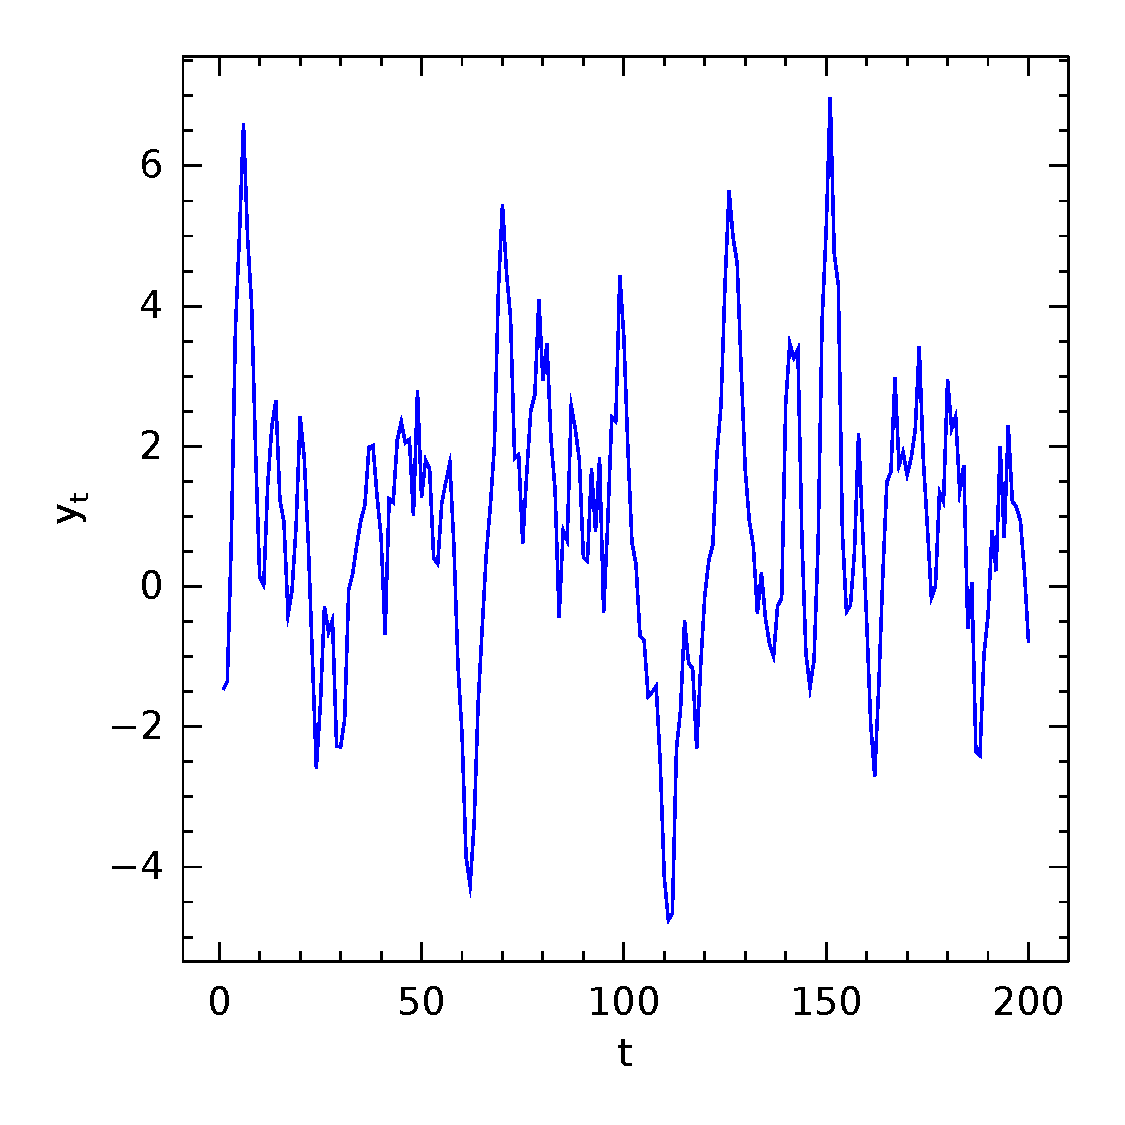
\includegraphics[width=0.7\linewidth]{Figuras/exemplo-yt}
\caption{Série temporal $y_t$}
\label{fig:exemployt}
\end{figure}

\begin{figure}[h]
\centering
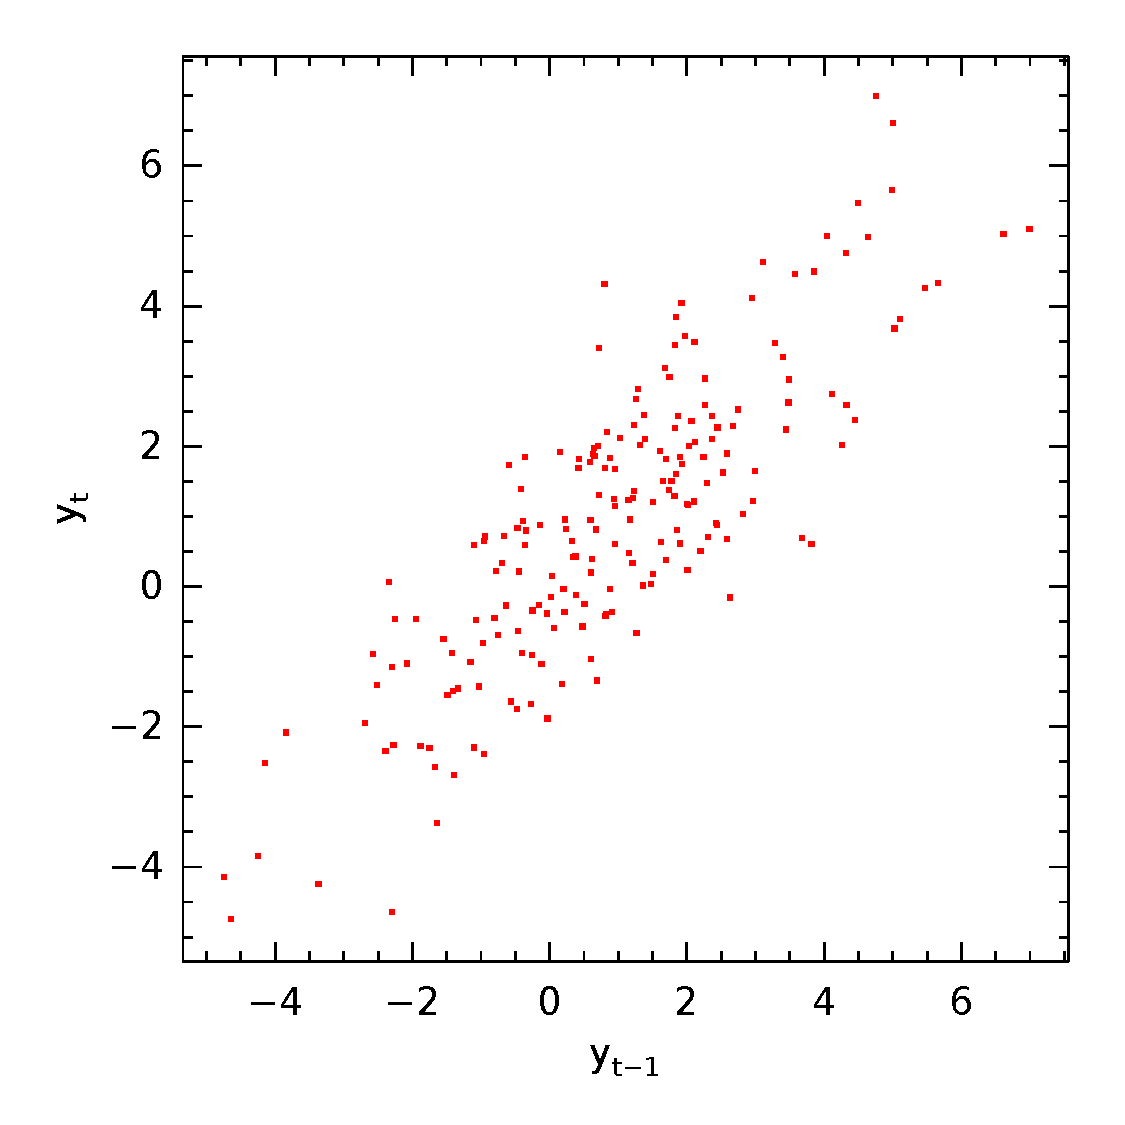
\includegraphics[width=0.7\linewidth]{Figuras/exemplo-ar}
\caption[Tst]{Relationship between $y_t$ and its first lag $y_{t-1}$}
\label{fig:exemploar}
\end{figure}

\todo[inline]{Refazer gráfico com pontos maiores}

Vamos investigar duas maneiras de estimar os quantis da relação acima: utilizando um modelo linear e um modelo não paramétrico.


\section{Estimando a QAR com um modelo linear}

Ao estimar um modelo de regressão quantílica, estamos interessados em encontrar uma função $f$ que minimize a soma dos erros
\begin{equation}
\min_{f}\sum_{i=1}^{n}\alpha|y_{t}-f(t)|^{+}+(1-\alpha)|y_{t}-f(t)|^{-},
\end{equation}
em que $|x|^+=\max\{0,x\}$ e $|x|^-=-\min\{0,x\}$.
Para resolver este problema como um problema de programação linear, podemos criar variáveis $\delta^+$ e $\delta^-$ para representar as funções $|\cdot|^+$ e $|\cdot|^-$, respectivamente, e montá-lo da seguinte forma:
\begin{equation}
\begin{aligned}\min_{f} & \sum_{i=1}^{n}\left(\lambda\delta_{i}^{+}+(1-\lambda)\delta_{i}^{-}\right)\\
\mbox{sujeito à } & \delta_{i}^{+}-\delta_{i}^{-}=y_{i}-f(x_{i}),\qquad\forall i\in\{1,\dots,n\},\\
& \delta_i^+,\delta_i^- \geq 0, \qquad \forall \{1,\dots,n\}.
\end{aligned}
\end{equation}

Quando assumimos que a função $f$ que estima o $\alpha$-ésimo quantil é uma função linear, tal que $f(x) = \beta_0 + \beta^T x$, os valores de $\beta_0$ e $\beta$ podem ser obtidos como sendo aqueles vindos da solução do seguinte problema de minimização:
\begin{equation}
\begin{aligned}\min_{\beta_0,\beta} & \sum_{i=1}^{n}\left(\alpha\delta_{i}^{+}+(1-\alpha)\delta_{i}^{-}\right)\\
\mbox{sujeito � } & \delta_{i}^{+}-\delta_{i}^{-}=y_{i} - \beta_0 - \beta^T x_{i},\qquad\forall i\in\{1,\dots,n\},\\
& \delta_i^+,\delta_i^- \geq 0, \qquad \forall \{1,\dots,n\}.
\end{aligned}
\end{equation}

%Utilizando um modelo linear de regressão quantílica para estimar os coeficientes do QAR %

\todo[inline]{Resultados para a estimação linear}

\section{Estimando a QAR não parametricamente}

Fitting a linear estimator for the Quantile Auto Regression isn't appropriate  when nonlinearity is present in the data. This nonlinearity may produce a linear estimator that underestimates the quantile for a chunk of data while overestimating for the other chunk (we illustrate this in figure \ref{fig:nonlinear}). To prevent this issue from occurring we propose a modification which we let the prediction $\mathcal{Q}_{y_t|y_{t-1}}^\alpha(t)$ adjust freely to the data and its nonlinearities. To prevent overfitting and smoothen our predictor, we include a penalty on its roughness by including the $\ell_1$ norm of its second derivative. For more information on the $\ell_1$ norm acting as a filter, one can refer to \cite{kim2009ell_1}.

\begin{figure}
\centering
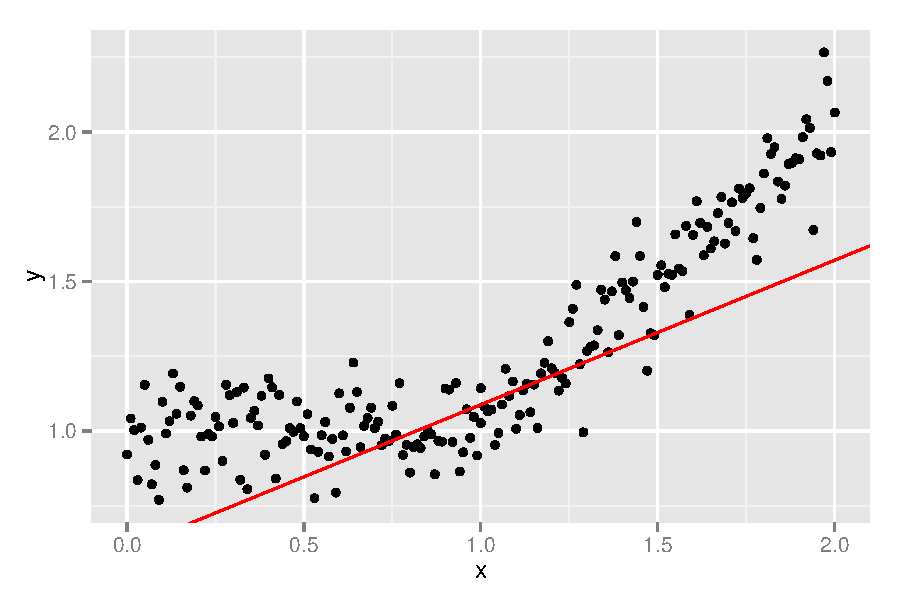
\includegraphics[width=0.7\linewidth]{../Paper_IEEE/nonlinear}
\caption{Example of data where nonlinearity is present and a linear quantile estimator is employed}
\label{fig:nonlinear}
\end{figure}


% notação estatística de ordem. com x^(0)

Let $\{\tilde{y}_t \}_{t=1}^n$ be the sequence of observations in time $t$. Now, let $\tilde{x}_t$ be the $p-$lagged time series of $\tilde{y}_t$, such that $\tilde{x}_t = L^p(\tilde{y}_t)$, where $L$ is the lag operator. Matching each observation $\tilde{y}_t$ with its $p-$lagged correspondent $\tilde{x}_t$ will produce $n-p$ pairs $\{(\tilde{y}_t,\tilde{x}_t)\}_{t=p+1}^n$ (note that the first $p$ observations of $y_t$ must be discarded). When we order the observation of $x$ in such way that they are in growing order
$$\tilde{x}_{(p+1)} \leq \tilde{x}_{(p+2)} \leq \dots \leq \tilde{x}_{(n)},$$ 
we can then define $\{x_i\}_{i=1}^{n-p} = \{\tilde{x}_{(t)} \}_{t=p+1}^{n}$ and $\{y_i\}_{i=1}^{n-p} = \{\tilde{y}_{(t)} \}_{t=p+1}^{n}$ and $I = \{2,\dots, n-p-1\}$. As we need the second difference of $q_i$, $I$ has to be shortened by two elements.

Our optimization model to estimate the nonparametric quantile is as follows:
\begin{equation}
\begin{split}
\mathcal{Q}_{y_t|y_{t-1}}^\alpha(i) =\underset{q_{i}}{\arg\min}\sum_{i\in I}\left(|y_{i}-q_{i}|^{+}\alpha + |y_{i}-q_{i}|^{-}(1-\alpha)\right) \\ +\lambda  \sum_{i\in I}|D^{2}q_{i}|,
\end{split}
\end{equation}
where $D^2 q_t$ is the second derivative of the $q_t$ function, calculated as follows:
\begin{equation*}
D^{2}q_{i}=\left(\frac{q_{i+1}-q_{i}}{x_{i+1}-x_{i}}\right)-\left(\frac{q_{i}-q_{i-1}}{x_{i}-x_{i-1}}\right).
\end{equation*}
The first part on the objective function is the usual quantile regression condition for $\{q_i\}$. The second part is the $\ell_1$-filter. The purpose of a filter is to control the amount of variation for our estimator $q_i$. When no penalty is employed we would always get $q_i = y_i$. On the other hand, when $\lambda \rightarrow \infty$, our estimator approaches the linear quantile regression.

The output of our optimization problem is a sequence of ordered points $\{(x_i, q_i)\}_{i \in I}$. The next step is to interpolate these points in order to provide an estimation for any other value of x. To address this issue, we propose a B-splines interpolation, that will be discussed in another subsection.

When estimating quantiles for a few different values of $\alpha$, however, sometimes we find them overlapping each other, which we call crossing quantiles. To prevent this, we include a non-crossing constraint:
\begin{equation}
q_i^{\alpha} \leq q_i^{\alpha'}, \quad \forall i \in I, \alpha < \alpha'.
\label{eq:non-crossing}
\end{equation} 

\todo[inline]{traduzir trecho acima}

Testamos a regressão quantílica não paramétrica para estimar quantis para diversos tipos de dados e de penalizações. A seguir, apresentamos o resultado da regressão quantílica para dados gerados a partir de um modelo ARIMA com diversos valores distintos de penalização, com ou sem a restrição de não-cruzamento de quantis. As figuras contém todos os quantis entre 1\% e 99\%.

\begin{figure}
\centering
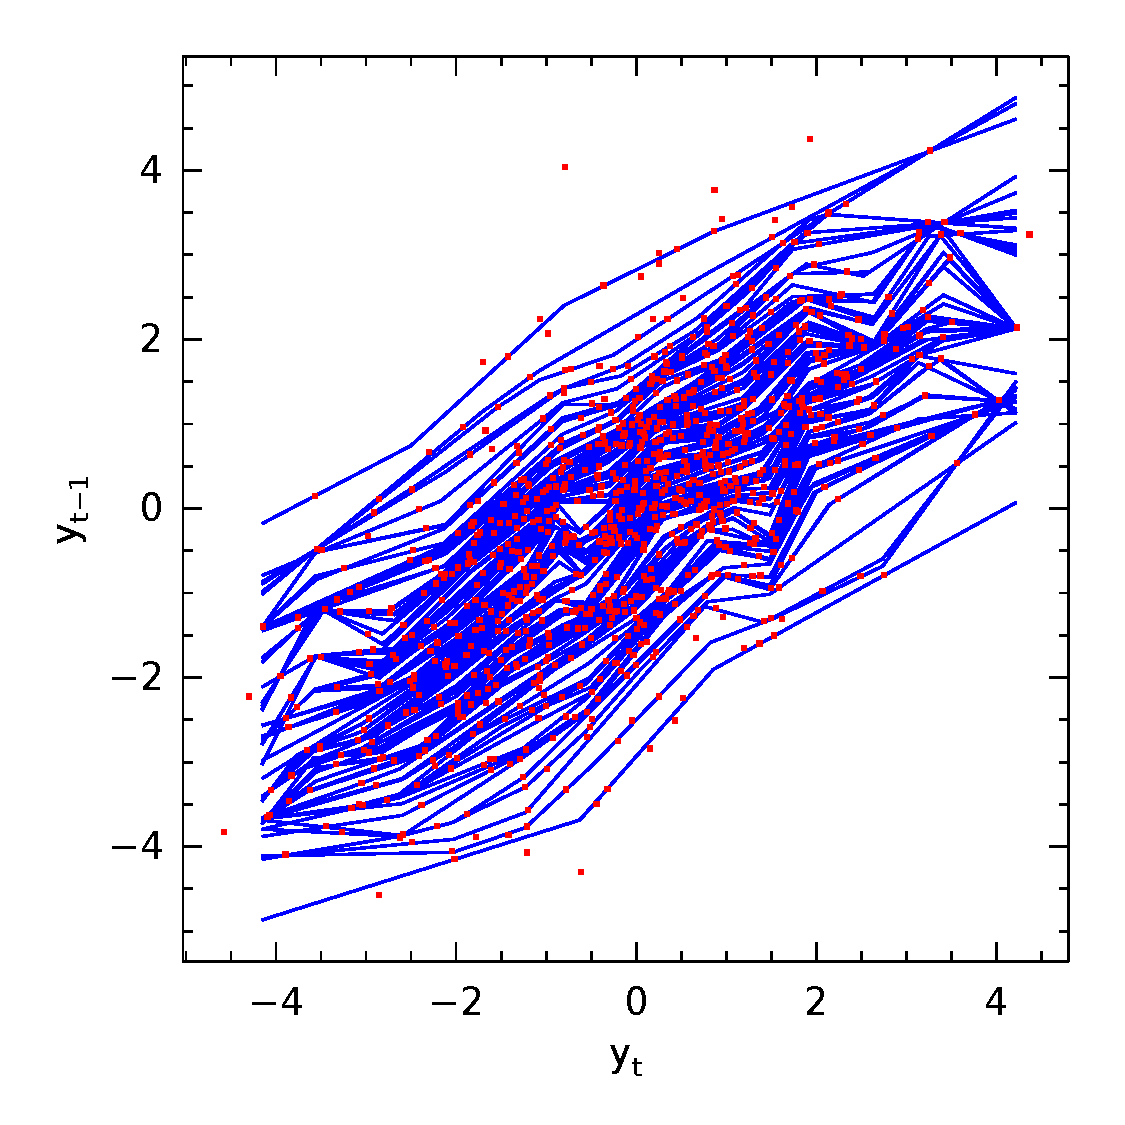
\includegraphics[width=0.6\linewidth]{Figuras/arima-crossing-03.pdf}
\caption{Dados simulados ARIMA com penalização $\lambda=0.3$}
\label{fig:arima-crossing-03}
\end{figure}

\begin{figure}
\centering
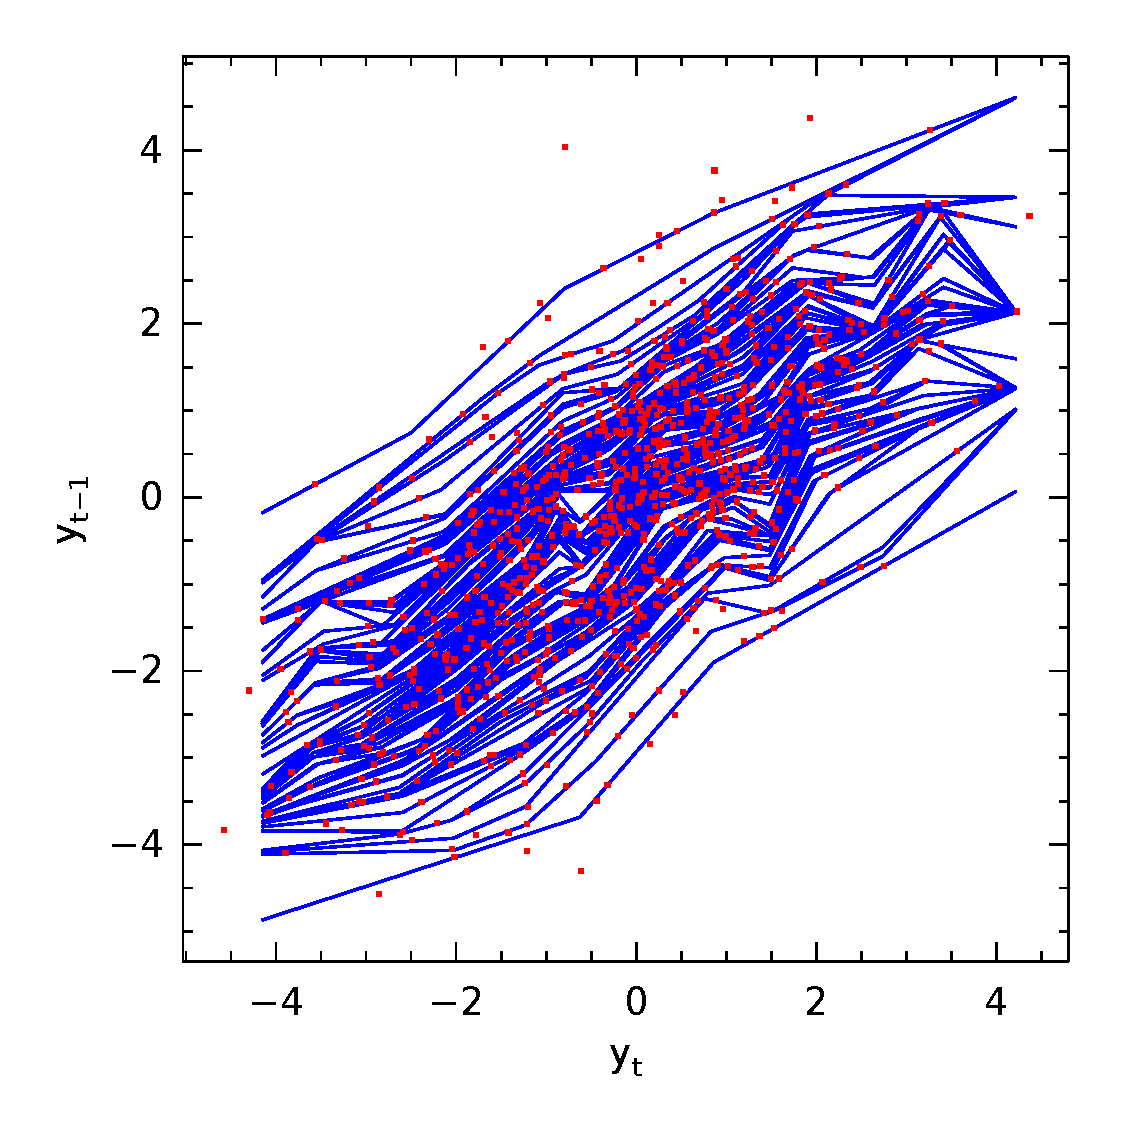
\includegraphics[width=0.5\linewidth]{Figuras/arima-noncrossing-03.pdf}
\caption{Dados simulados ARIMA com penalização $\lambda=0.3$ e restrição de não cruzamento de quantis}
\label{fig:arima-noncrossing-03}
\end{figure}

\begin{figure}
\centering
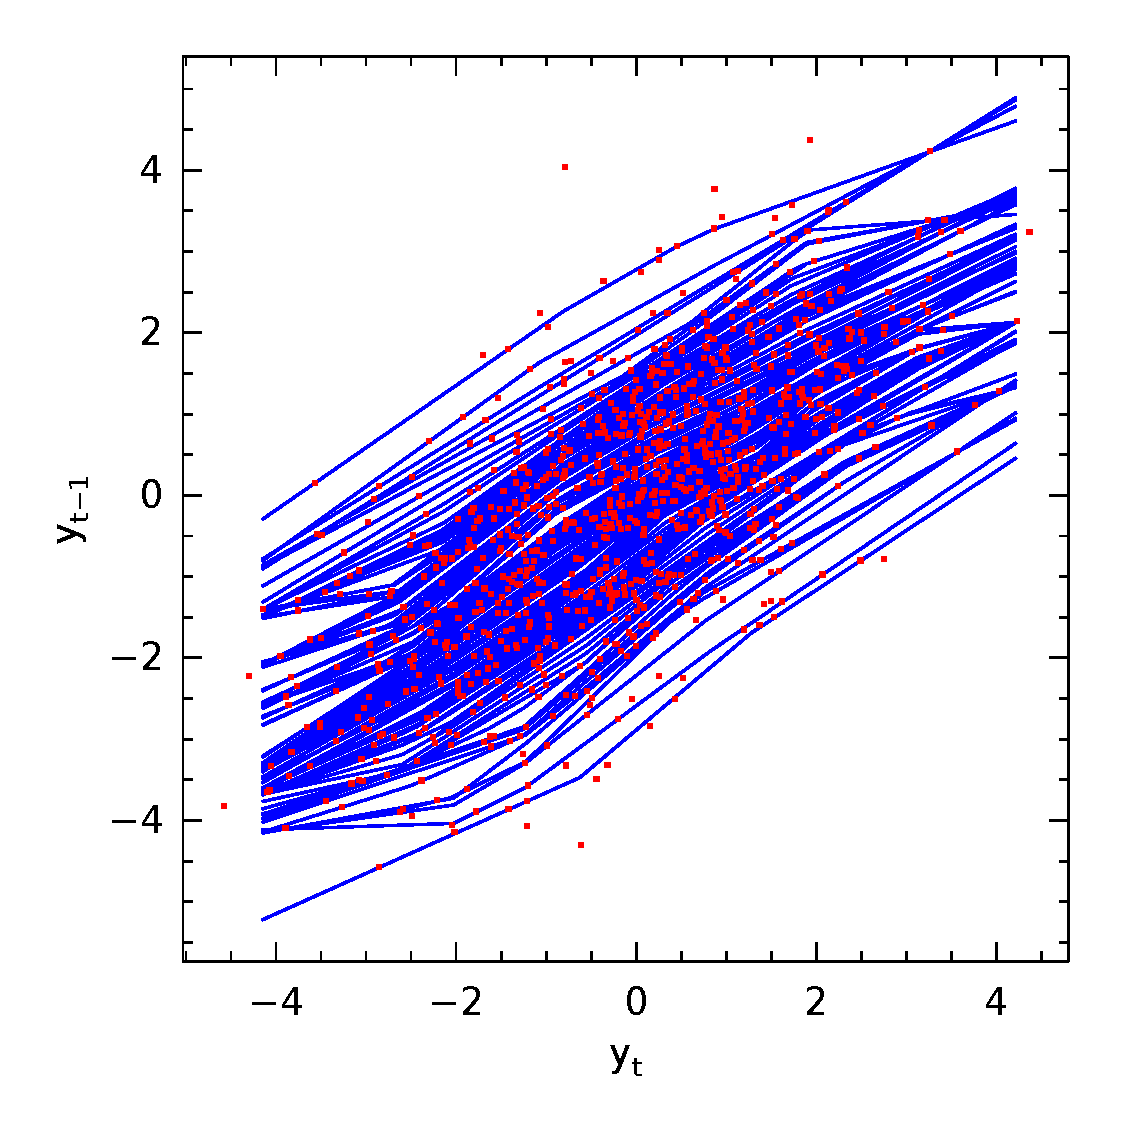
\includegraphics[width=0.6\linewidth]{Figuras/arima-crossing-1.pdf}
\caption{Dados simulados ARIMA com penalização $\lambda=1$}
\label{fig:arima-crossing-1}
\end{figure}

\begin{figure}
\centering
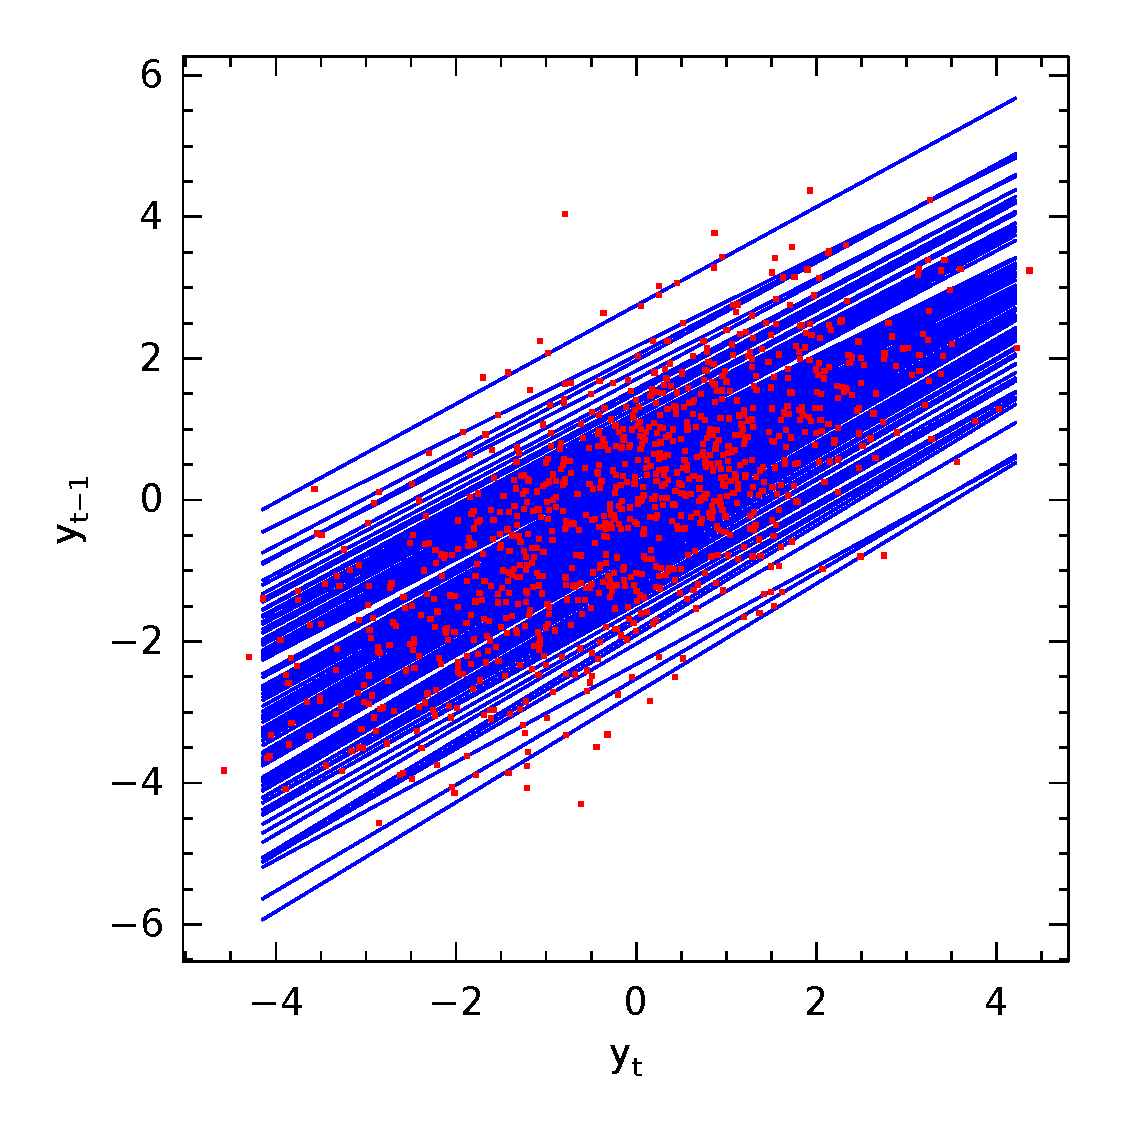
\includegraphics[width=0.5\linewidth]{Figuras/arima-crossing-10.pdf}
\caption{Dados simulados ARIMA com penalização $\lambda=10$}
\label{fig:arima-crossing-10}
\end{figure}

Na estimação com valor de $\lambda=0.3$ (figura \ref{fig:arima-crossing-03}), observamos que a estimação do quantil possui uma variância muito alta. Nesses casos, o erro \textit{in-sample} é baixo, mas as previsões serão muito ruins. À medida que o valor incrementamos o valor de $\lambda$ (figura \ref{fig:arima-crossing-1}, onde utilizamos $\lambda=1$), a função estimada para os quantis fica cada vez mais próxima de uma função linear, até que para valores mais extremos de $lambda$ (ver figura \ref{fig:arima-crossing-10}, onde utilizamos $\lambda=10$) ela será totalmente linear.

A restrição \ref{eq:non-crossing}, ao forçar que a função de nenhum quantil se cruze, produz uma diferença nos valores estimados. Esta diferença, no entanto, é perceptível apenas nas extremidades dos gráficos. As figuras \label{fig:arima-noncrossing-03} e \label{fig:arima-crossing-03} exemplificam as diferenças da inclusão ou não desta restrição.

%A seguir, apresentaremos alguns resultados para quando o 

%The difference between using or not this constraint can be seen in the two plots below:
%
%
%
%\bibliography{QR}
%\bibliographystyle{ieeetr}
%
%\end{document}

\clearpage
\bibliographystyle{plain}
\bibliography{QR}

\end{document}



% Jeremie Juban , Lionel Fugon, George Kariniotakis (2007): Probabilistic short- term wind power forecasting based on kernel density estimators. European Wind Energy Conference. (QR Forests)
% http://www.casact.org/education/rpm/2010/handouts/CL1-Fu.pdf
% http://mathematicaforprediction.wordpress.com/category/quantile-regression/
